\section{Results}
\label{sec:results}

Table~\ref{tab:maincompact} summarises every panel (full detail in Appendix Table~\ref{tab:main}); Table~\ref{tab:paired} the frozen paired comparisons; Figure~\ref{fig:op} the accuracy--cost operating points.
All frontier calls completed without failures except 25 Claude refusals on RewardBench, which are scored incorrect.
Total API spend for the whole study, including development, probes and ablations, was \$\ApiTotal.

\begin{table}[t]
\centering\small
\caption{Accuracy (\%) and, in parentheses, USD per 1{,}000 decisions on every panel (full table with intervals, failures and token counts: Appendix Table~\ref{tab:main}). JEV-9B S2 is run on every item only where it is a confirmatory arm (A6). $^\dagger$349 of 620 rows (A5).}
\label{tab:maincompact}
\resizebox{\linewidth}{!}{%
\begin{tabular}{@{}lcccccc@{}}
\toprule
System & FOLIO & ANLI r3 & Controlled & JudgeBench$^\dagger$ & RewardBench & HaluEval-QA \\
\midrule
JEV-9B S1 & 69.6 \scriptsize(0.041) & 64.2 \scriptsize(0.045) & 55.9 \scriptsize(0.037) & 68.2 \scriptsize(0.153) & 87.0 \scriptsize(0.170) & 82.7 \scriptsize(0.096) \\
JEV-9B S2 & 85.8 \scriptsize(0.609) & -- & 100.0 \scriptsize(0.609) & -- & -- & -- \\
JEV-H harness & 84.3 \scriptsize(0.483) & 74.6 \scriptsize(0.623) & 96.9 \scriptsize(0.572) & 88.2 \scriptsize(1.19) & 94.4 \scriptsize(0.654) & 87.7 \scriptsize(0.424) \\
Astra (high) & 86.8 \scriptsize(8.97) & 74.9 \scriptsize(7.00) & 100.0 \scriptsize(5.65) & 94.5 \scriptsize(22.01) & 93.8 \scriptsize(4.01) & 90.6 \scriptsize(2.45) \\
Fable (high) & 90.2 \scriptsize(11.68) & 77.3 \scriptsize(7.52) & 100.0 \scriptsize(7.87) & 94.2 \scriptsize(42.28) & 90.2 \scriptsize(5.78) & 93.3 \scriptsize(3.64) \\
\bottomrule
\end{tabular}}
\end{table}

\begin{table*}[t]
\centering\small
\caption{Paired comparisons of JEV-9B System~1 with each frontier (judge track: preregistration A3, $\alpha=0.05/4$). $\Delta$ = JEV-9B minus frontier accuracy (points).
Intervals are Bonferroni-adjusted within family (primary: $\alpha=0.05/4$; secondary: $\alpha=0.05/6$); cluster bootstrap where clusters repeat, Newcombe paired score interval otherwise.
Discordant = items only JEV-9B / only the frontier got right. Conclusions follow the frozen rule with a 2-point margin.}
\label{tab:paired}
\begin{tabular}{@{}lllrrrcl@{}}
\toprule
Family & Panel & Frontier & Clusters & Discordant & $\Delta$ & Adj.\ CI & Conclusion \\
\midrule
Primary & FOLIO & Astra (high) & 73 & 8/43 & -17.2 & [-26.6, -7.2] & frontier better \\
 & FOLIO & Fable (high) & 73 & 3/45 & -20.6 & [-29.0, -12.1] & frontier better \\
 & ANLI r3 & Astra (high) & 1128 & 96/224 & -10.7 & [-14.1, -7.0] & frontier better \\
 & ANLI r3 & Fable (high) & 1128 & 94/251 & -13.1 & [-16.7, -9.4] & frontier better \\
\midrule
Secondary & JudgeBench (partial) & Astra (high) & 157 & 11/102 & -26.3 & [-32.8, -17.2] & frontier better \\
 & JudgeBench (partial) & Fable (high) & 157 & 11/101 & -26.0 & [-32.2, -16.5] & frontier better \\
\midrule
Judge track & RewardBench & Astra (high) & 492 & 17/44 & -5.4 & [-9.4, -1.6] & inconclusive \\
 & RewardBench & Fable (high) & 492 & 37/46 & -1.8 & [-6.4, 2.6] & inconclusive \\
 & HaluEval-QA & Astra (high) & 1000 & 10/89 & -7.9 & [-10.4, -5.5] & frontier better \\
 & HaluEval-QA & Fable (high) & 1000 & 5/111 & -10.6 & [-13.3, -8.1] & frontier better \\
\bottomrule
\end{tabular}
\end{table*}


\begin{figure}[t]
\centering
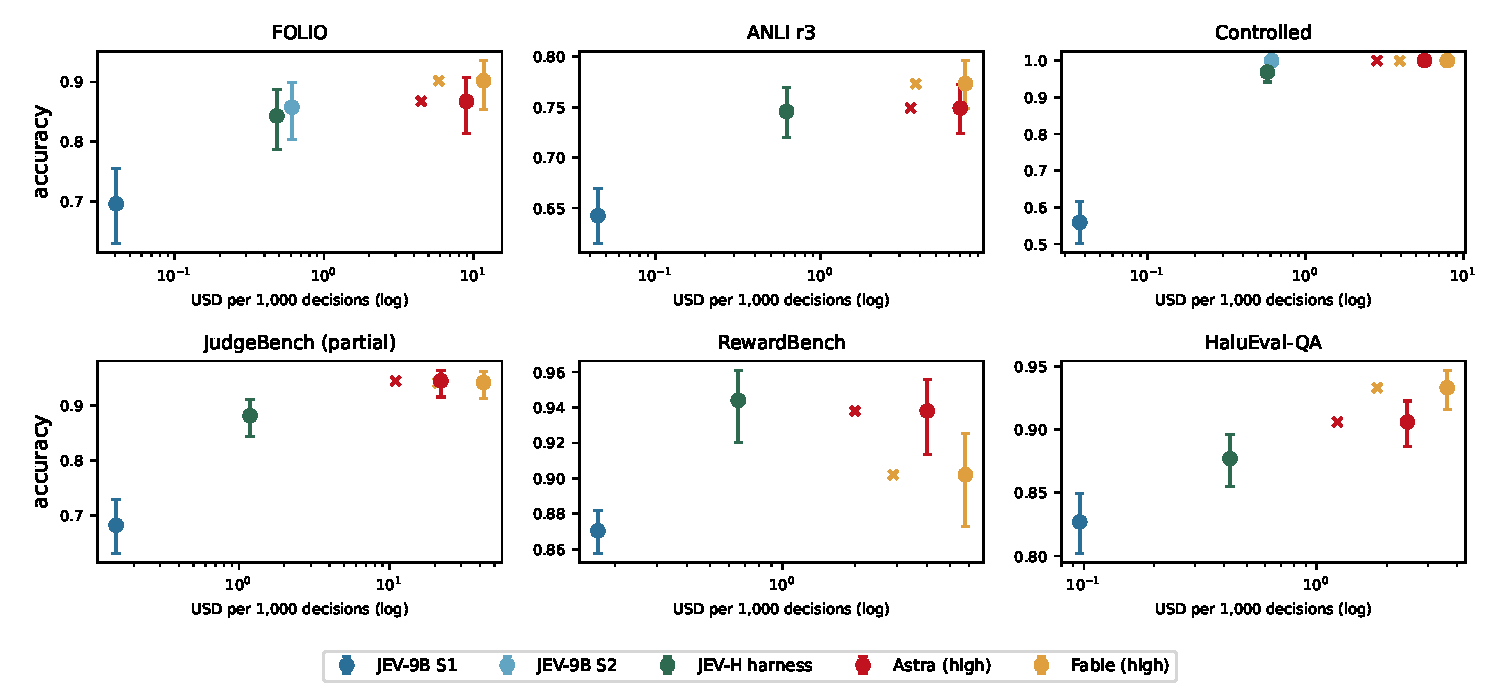
\includegraphics[width=\linewidth]{figures/operating_points.pdf}
\caption{Accuracy (95\% Wilson interval) against cost per 1{,}000 decisions (log scale). Circles: measured synchronous list price; crosses: the same frontier usage at batch prices. JEV-9B sits 25--290 times to the left of both frontiers.}
\label{fig:op}
\end{figure}

\subsection{Public reasoning panels: the frontiers are materially more accurate}
\label{sec:public}
On both primary panels the frozen rule returns \emph{frontier materially more accurate} against both providers (Table~\ref{tab:paired}).
On FOLIO, JEV-9B System~1 is correct on \AccFolioSone\% of items against \AccFolioAstra\% for Astra and \AccFolioFable\% for Fable ($\Delta=\DeltaFolioAstra$ and $\DeltaFolioFable$ points; adjusted upper bounds \HiFolioAstra{} and \HiFolioFable{}).
On ANLI round 3 the gaps are \DeltaAnliAstra{} and \DeltaAnliFable{} points, with upper bounds of \HiAnliAstra{} and \HiAnliFable{}: even the most favourable end of each interval is far outside the two-point margin.
The cost difference runs the other way by a similar order: \$\CostFolioSone{} per thousand FOLIO decisions for JEV-9B against \$\CostFolioAstra{} and \$\CostFolioFable{} for the frontiers.
Neither frontier was close to its output budget: mean output, including reasoning, was 49--137 tokens per item at \texttt{high} effort.

\paragraph{The same weights, thinking, close most of the gap.}
JEV-9B System~2---the identical backbone with its reasoning enabled---reaches \AccFolioStwo\% on FOLIO, within a point of Astra (\AccFolioAstra\%), at \$\CostFolioStwo{} per thousand decisions (Table~\ref{tab:main}).
The deficit of the one-pass decision path is therefore not a deficit of the backbone's knowledge: the information needed is in the weights, and a single forward pass does not extract it.

\subsection{The controlled panel: not depth, but the absence of a derivation}
\label{sec:controlled-results}
\begin{table}[t]
\centering\small
\caption{Controlled panel accuracy (\%) by dependency depth $d$ and irrelevant facts $c$ (48 seeds per cell), and by gold label (96 items each). Chance is 33\%.}
\label{tab:cells}
\begin{tabular}{@{}lcccccc|ccc@{}}
\toprule
& \multicolumn{2}{c}{$d=1$} & \multicolumn{2}{c}{$d=3$} & \multicolumn{2}{c|}{$d=5$} & \multicolumn{3}{c}{Gold label} \\
System & $c{=}0$ & $c{=}8$ & $c{=}0$ & $c{=}8$ & $c{=}0$ & $c{=}8$ & True & False & Unk. \\
\midrule
JEV-9B S1 & 60 & 62 & 60 & 40 & 67 & 46 & 62 & 80 & 25 \\
JEV-9B S2 & 100 & 100 & 100 & 100 & 100 & 100 & 100 & 100 & 100 \\
JEV-H harness & 98 & 98 & 94 & 98 & 96 & 98 & 99 & 98 & 94 \\
Astra (high) & 100 & 100 & 100 & 100 & 100 & 100 & 100 & 100 & 100 \\
Fable (high) & 100 & 100 & 100 & 100 & 100 & 100 & 100 & 100 & 100 \\
\bottomrule
\end{tabular}
\end{table}

\begin{table}[t]
\centering\small
\caption{Depth and distractor interactions on the controlled panel (points). $\Delta_J$, $\Delta_F$: change in JEV-9B~S1 and comparator accuracy between levels; DID $=\Delta_J-\Delta_F$. H1: Bonferroni $\alpha=0.05/6$; H1c (same-weights System~2 comparator): $\alpha=0.05$. Cluster bootstrap over 48 seeds. \checkmark: interval excludes 0.}
\label{tab:did}
\begin{tabular}{@{}lllrrrcc@{}}
\toprule
Fam. & Comparator & Contrast & $\Delta_J$ & $\Delta_F$ & DID & Adj.\ CI & \\
\midrule
H1 & Astra (high) & depth 5 vs 1 & -5.2 & 0.0 & -5.2 & [-24.0, 13.5] &  \\
H1 & Astra (high) & depth 3 vs 1 & -11.5 & 0.0 & -11.5 & [-28.1, 6.2] &  \\
H1 & Astra (high) & distractors 8 vs 0 & -13.2 & 0.0 & -13.2 & [-27.1, 0.7] &  \\
H1 & Fable (high) & depth 5 vs 1 & -5.2 & 0.0 & -5.2 & [-24.0, 13.5] &  \\
H1 & Fable (high) & depth 3 vs 1 & -11.5 & 0.0 & -11.5 & [-28.1, 6.2] &  \\
H1 & Fable (high) & distractors 8 vs 0 & -13.2 & 0.0 & -13.2 & [-27.1, 0.7] &  \\
H1c & JEV-9B S2 & depth 5 vs 1 & -5.2 & 0.0 & -5.2 & [-18.8, 8.3] &  \\
H1c & JEV-9B S2 & depth 3 vs 1 & -11.5 & 0.0 & -11.5 & [-24.0, 1.0] &  \\
\bottomrule
\end{tabular}
\end{table}

\begin{table}[t]
\centering\small
\caption{Paired controls at $d{=}3$, $c{=}8$ (48 seeds, \%). Changing: one verified edit flips the gold label. Preserving: renamed entities and reordered premises, same label. ``Changed'' = answer differs from the base answer; ``Both'' = correct on base and edited item; ``Invariant'' = same answer as base.}
\label{tab:controls}
\begin{tabular}{@{}lrrrrrr@{}}
\toprule
& Base & \multicolumn{3}{c}{Decision-changing} & \multicolumn{2}{c}{Decision-preserving} \\
System & acc. & acc. & changed & both & acc. & invariant \\
\midrule
JEV-9B S1 & 40 & 58 & 48 & 23 & 31 & 58 \\
JEV-9B S2 & 100 & 100 & 100 & 100 & 100 & 100 \\
JEV-H harness & 98 & 98 & 98 & 96 & 98 & 96 \\
Astra (high) & 100 & 100 & 100 & 100 & 100 & 100 \\
Fable (high) & 100 & 100 & 100 & 100 & 100 & 100 \\
\bottomrule
\end{tabular}
\end{table}


Every reasoning system---both frontiers and JEV-9B System~2---answers all 288 base items correctly at every depth and context (Table~\ref{tab:cells}); the fragment is easy for any system that reasons.
JEV-9B System~1 is correct on \AccCtlSone\%.
Our primary hypothesis H1 predicted that this deficit would grow with dependency depth.
\textbf{It did not, at our precision.}
Moving from depth~1 to depth~5 changes System~1 accuracy by \ChgAstraDfive{} points, a difference-in-differences of \DidAstraDfive{} against either frontier with an adjusted interval of [\DidLoAstraDfive, \DidHiAstraDfive] (Table~\ref{tab:did}); depth~3 gives \DidAstraDthree{} [\DidLoAstraDthree, \DidHiAstraDthree].
Neither interval excludes zero, so H1 is not supported; with 48 seeds we cannot exclude a moderate depth effect either.
The eight irrelevant facts, which add about 250 characters, move accuracy by \DidAstraCtx{} points [\DidLoAstraCtx, \DidHiAstraCtx]---a larger point estimate than depth, contrary to H1b, though its interval also touches zero.

The structure of the errors is clearer than their dependence on depth.
By gold label (Table~\ref{tab:cells}, right), System~1 is correct on most \emph{False} items and on a majority of \emph{True} items, but on only a quarter of \emph{Unknown} items: it rarely concludes that nothing follows.
Its predictions are also unstable under edits that should not matter: renaming entities and reordering premises preserves its answer on only \CtlSoneInvariant\% of seeds, against 100\% for every reasoning system (Table~\ref{tab:controls}).
And under an edit that flips the verified label, it changes its answer on \CtlSoneAnswerChanged\% of seeds and is right on both the original and the edited item on only \CtlSoneBothCorrect\%.
Together these say that, on this fragment, the one-pass model is not tracking the derivation at all: it reads surface cues, and the cue it most lacks is the one for ``no rule applies''.

The deep extension (A1; 12 rules, depths 1/5/9, exploratory) shows the same picture with more room: System~1 scores \DeepSoneDOne\%, \DeepSoneDFive\% and \DeepSoneDNine\% at depths 1, 5 and 9, System~2 \DeepStwoDOne\%, \DeepStwoDFive\% and \DeepStwoDNine\%, and both frontiers 100\% throughout (Figure~\ref{fig:depth}).
Even at nine dependent steps the frontier models do not drop an item; whatever their depth limit is, it lies beyond what a 12-rule, sub-1{,}000-character problem can probe.

\begin{figure}[t]
\centering
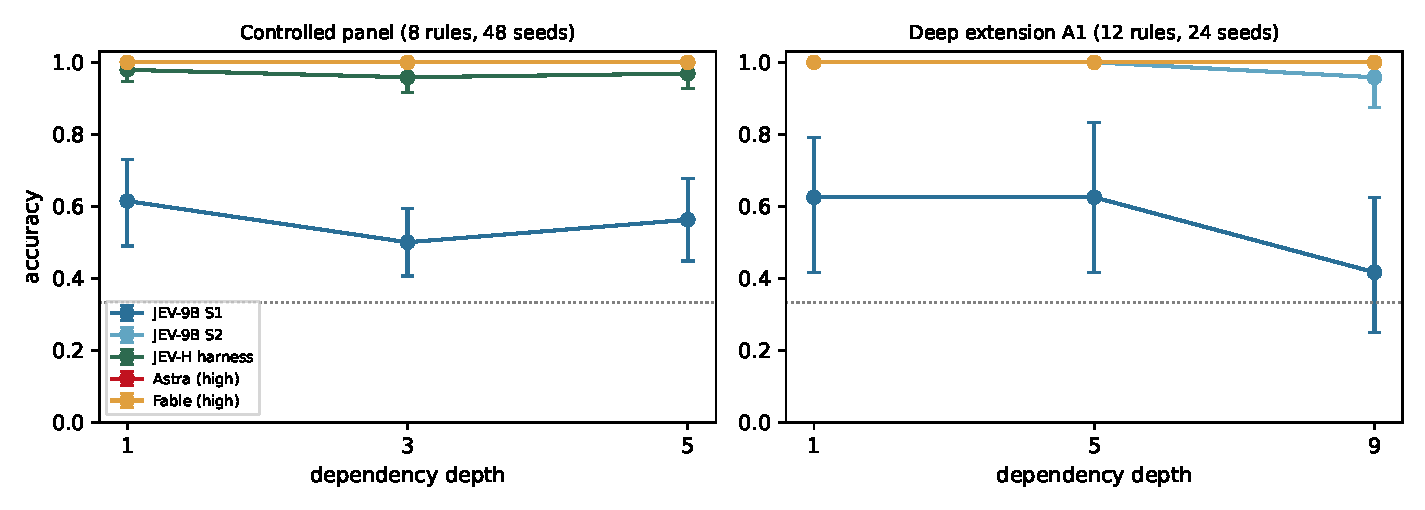
\includegraphics[width=\linewidth]{figures/depth.pdf}
\caption{Accuracy by dependency depth with seed-clustered 95\% bootstrap intervals. Left: the preregistered controlled panel (8 rules, depths 1/3/5). Right: the exploratory deep extension (12 rules, depths 1/5/9). Dotted line: chance.}
\label{fig:depth}
\end{figure}

\paragraph{Same weights, different computation (H1c).}
Against its own System~2, System~1's depth-3-versus-depth-1 difference-in-differences is \DidStwoDthree{} points [\DidLoStwoDthree, \DidHiStwoDthree] and depth-5-versus-1 is \DidStwoDfive{} [\DidLoStwoDfive, \DidHiStwoDfive].
Because System~2 is flat at 100\%, these contrasts mostly restate System~1's own variation; the more informative statement is the level: identical weights solve every controlled item when allowed to reason, and solve \AccCtlSone\% when not.

\subsection{Judging LLM outputs}
\label{sec:judging}
\begin{table}[t]
\centering\small
\caption{RewardBench (2{,}985 filtered pairs) accuracy (\%) by official section; ``Score'' is the unweighted section mean, ``All'' the item mean. HaluEval-QA answer-length-only AUROC (trivial baseline): 0.976.}
\label{tab:judgetrack}
\begin{tabular}{@{}lrrrrrr@{}}
\toprule
System & Chat & Chat Hard & Safety & Reasoning & Score & All \\
\midrule
JEV-9B S1 & 96.4 & 67.5 & 90.1 & 89.3 & 85.8 & 87.0 \\
JEV-9B S2 & 81.8 & 83.7 & 87.2 & 98.6 & 87.8 & 92.2 \\
JEV-H harness & 93.3 & 81.7 & 94.0 & 98.7 & 91.9 & 94.4 \\
Astra (high) & 86.7 & 84.5 & 91.0 & 100.0 & 90.5 & 93.8 \\
Fable (high) & 96.7 & 87.3 & 71.4 & 100.0 & 88.9 & 90.2 \\
\bottomrule
\end{tabular}
\end{table}

\begin{table}[t]
\centering\small
\caption{Accuracy (\%) on inputs of at most / more than 1{,}024 JEV-9B tokens, the length on which JEV-9B was trained. Only panels with long inputs are shown.}
\label{tab:length}
\begin{tabular}{@{}lcccccc@{}}
\toprule
Panel & $n$ short/long & JEV-9B S1 & JEV-9B S2 & JEV-H & Astra & Fable \\
\midrule
JudgeBench (partial) & 54 / 292 & 64.8 / 68.8 & 73.5 / 87.9 & 87.0 / 88.4 & 88.9 / 95.5 & 94.4 / 94.2 \\
RewardBench & 2778 / 206 & 87.2 / 85.0 & 92.4 / 89.5 & 94.3 / 96.4 & 93.9 / 92.9 & 89.8 / 96.4 \\
\bottomrule
\end{tabular}
\end{table}


The judge track asks whether JEV-9B can replace a frontier LLM-as-a-judge.
\textbf{On RewardBench it is the closest to parity of any panel.}
One-pass JEV-9B is correct on \AccRbSone\% of all 2{,}985 filtered pairs; on the sealed 500-pair sample shared with the frontiers it trails Astra by \DeltaRbAstra{} points [\LoRbAstra, \HiRbAstra] and Fable by only \DeltaRbFable{} points [\LoRbFable, \HiRbFable] (Table~\ref{tab:paired}).
Against Fable the interval includes zero but not the full two-point margin, so the frozen rule returns \emph{inconclusive}: we can neither certify noninferiority nor show a difference.
By section (Table~\ref{tab:judgetrack}), JEV-9B matches Fable on Chat (\RbSoneChat\% vs.\ \RbFableChat\%) and \emph{exceeds} it on Safety (\RbSoneSafety\% vs.\ \RbFableSafety\%), where Fable's refusals to adjudicate harmful prompts count against it; it is clearly weaker on Chat Hard (\RbSoneChatHard\% vs.\ \RbFableChatHard\%), the adversarial instruction-following pairs, and on Reasoning (\RbSoneReasoning\% vs.\ 100\%).
It does this at \$\CostRbSone{} per thousand judgements, against \$\CostRbAstra{} and \$\CostRbFable.

On JudgeBench---difficult, mostly long correctness judgements---the gap is large (\DeltaJbgptAstra{} and \DeltaJbgptFable{} points on the GPT-response split; the Claude split has too few completed rows to analyse, Appendix~\ref{app:prereg}).
On HaluEval-QA JEV-9B detects hallucinated answers at \AccHaluSone\%, against \AccHaluAstra\% and \AccHaluFable\% (gaps \DeltaHaluAstra{} and \DeltaHaluFable).
\emph{All three judges are below a trivial baseline here}: answer length alone separates right from hallucinated answers with AUROC \HaluLenAuroc, because HaluEval's hallucinated answers are systematically longer.
We report HaluEval for completeness but draw no conclusion about hallucination detection from it.



\subsection{Is the one-pass probability calibrated?}
\label{sec:calibration}
\begin{table}[t]
\centering\small
\caption{Calibration of JEV-9B System~1's top probability by task family: mean confidence, accuracy, their gap (overconfidence, points) and expected calibration error (15 bins).}
\label{tab:calibration}
\begin{tabular}{@{}lrrrrr@{}}
\toprule
Family & $n$ & Mean conf. & Accuracy & Over-conf. & ECE \\
\midrule
anli & 1200 & 73.0 & 64.2 & 8.8 & 0.105 \\
controlled & 488 & 66.9 & 56.1 & 10.7 & 0.116 \\
folio & 204 & 76.4 & 69.6 & 6.8 & 0.098 \\
halueval & 1000 & 89.0 & 82.7 & 6.3 & 0.067 \\
judgebench & 349 & 75.5 & 68.2 & 7.3 & 0.085 \\
rewardbench & 2984 & 88.5 & 87.0 & 1.5 & 0.026 \\
\bottomrule
\end{tabular}
\end{table}

\begin{figure}[t]
\centering
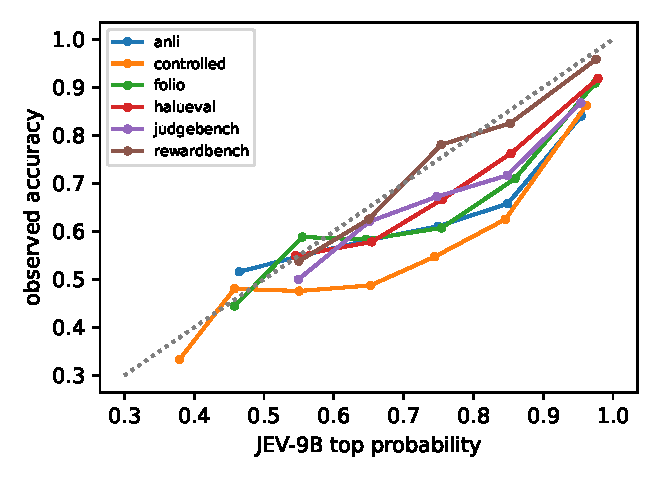
\includegraphics[width=0.55\linewidth]{figures/calibration.pdf}
\caption{Reliability of JEV-9B System~1's top probability by task family (bins with at least 15 items).}
\label{fig:calibration}
\end{figure}
A decision model's selling point is its probability, so we test it out of distribution (Table~\ref{tab:calibration}, Figure~\ref{fig:calibration}).
On RewardBench the top probability is well calibrated (mean confidence 88.5\% against 87.0\% accuracy; ECE 0.026).
On the reasoning panels it is systematically overconfident by 6.8 (FOLIO) to 10.7 (controlled) points, with ECE around 0.10---two orders of magnitude above the 0.0007 the model card reports on its in-distribution test set.
Confidence remains informative for ranking (it is what makes the JEV-H gate work), but a deployment should not read a 0.8 from JEV-9B on a reasoning task as an 80\% chance of being right without recalibrating on its own data.

\subsection{The JEV-H harness}
\label{sec:harness-results}
\begin{table*}[t]
\centering\small
\caption{JEV-H harness (A4: two option orders, threshold 0.90 fixed a priori, escalation to JEV-9B's own System~2) against each frontier. $\Delta$ = JEV-H minus frontier (points); intervals Bonferroni-adjusted over all 12 panel $\times$ frontier pairs. $^\dagger$Not preregistered: all 25 of Claude Fable's RewardBench refusals are Safety pairs, scored incorrect in the primary row; this row drops them.}
\label{tab:harness}
\resizebox{\linewidth}{!}{\begin{tabular}{@{}llrrrcl@{}}
\toprule
Panel & Frontier & JEV-H & Frontier & $\Delta$ & Adj.\ CI & Conclusion \\
\midrule
FOLIO & Astra (high) & 84.3 & 86.8 & -2.5 & [-9.6, 5.1] & inconclusive \\
 & Fable (high) & 84.3 & 90.2 & -5.9 & [-12.9, 0.0] & inconclusive \\
ANLI r3 & Astra (high) & 74.6 & 74.9 & -0.3 & [-3.9, 3.1] & inconclusive \\
 & Fable (high) & 74.6 & 77.3 & -2.8 & [-6.1, 0.6] & inconclusive \\
Controlled & Astra (high) & 96.9 & 100.0 & -3.1 & [-6.2, -0.7] & inconclusive \\
 & Fable (high) & 96.9 & 100.0 & -3.1 & [-6.2, -0.7] & inconclusive \\
JudgeBench (partial) & Astra (high) & 88.2 & 94.5 & -6.4 & [-19.1, -1.5] & inconclusive \\
 & Fable (high) & 88.2 & 94.2 & -6.1 & [-16.6, -1.9] & inconclusive \\
RewardBench & Astra (high) & 94.4 & 93.8 & 0.6 & [-2.4, 3.6] & inconclusive \\
 & Fable (high) & 94.4 & 90.2 & 4.2 & [0.4, 8.2] & JEV-H better \\
HaluEval-QA & Astra (high) & 87.7 & 90.6 & -2.9 & [-5.3, -0.7] & inconclusive \\
 & Fable (high) & 87.7 & 93.3 & -5.6 & [-8.2, -3.3] & frontier better \\
\addlinespace
RewardBench, refusals excluded$^\dagger$ & Fable (high) & 94.1 & 94.9 & -0.8 & [-4.0, 2.1] & sensitivity only ($n=475$) \\
\bottomrule
\end{tabular}}
\end{table*}


JEV-H (preregistration A4) asks System~1 in both option orders and escalates to System~2 when the averaged confidence is below 0.90; it has no fitted parameter.
Its escalation rate is itself informative: \EscHalueval\% of HaluEval, \EscRewardbench\% of RewardBench, \EscFolio\% of FOLIO, \EscAnli\% of ANLI and \EscJudgebench\% of JudgeBench items fall below the threshold, so the one-pass model is confident mostly where it is accurate.
Table~\ref{tab:harness} compares the harness with each frontier in its own Bonferroni family of 12 comparisons.

\textbf{On RewardBench the harness is the most accurate system we tested.}
It is correct on \AccRbHarn\% of the 500 shared pairs, against \AccRbAstra\% for Astra ($\Delta=\DeltaHRbAstra$ [\LoHRbAstra, \HiHRbAstra]) and \AccRbFable\% for Fable ($\Delta=\DeltaHRbFable$ [\LoHRbFable, \HiHRbFable]).
Under the preregistered scoring the frozen rule returns \emph{\ConclHRbFable} against Fable.
That verdict needs one qualification, which we state as prominently as the result: all 25 of Fable's refusals are Safety pairs, scored as errors.
On the 475 pairs Fable answered, JEV-H and Fable are statistically indistinguishable (\AccHRbFableAnsweredH\% vs.\ \AccHRbFableAnsweredF\%, $\Delta=\DeltaHRbFableAnswered$ [\LoHRbFableAnswered, \HiHRbFableAnswered]; a sensitivity analysis that was not preregistered).
Against Astra the interval sits within $[-2.4, 3.6]$: the harness neither loses nor certifiably matches it under the two-point margin.
It does this at \$\CostRbHarn{} per thousand judgements, against \$\CostRbAstra{} and \$\CostRbFable.

On the reasoning panels the harness recovers most of the one-pass deficit.
On ANLI it is \AccAnliHarn\% against Astra's \AccAnliAstra\% ($\Delta=\DeltaHAnliAstra$ [\LoHAnliAstra, \HiHAnliAstra]), up from System~1's \AccAnliSone\%; on FOLIO \AccFolioHarn\% against \AccFolioAstra\%; on the controlled panel \AccCtlHarn\%.
None of these reach the frozen rule's \emph{comparable} verdict---their lower bounds pass the two-point margin---but none is a material frontier advantage either, where System~1 alone was.
The harness still trails clearly on HaluEval (\AccHaluHarn\% vs.\ \AccHaluFable\% for Fable) and on JudgeBench (\AccJbgptHarn\% vs.\ \AccJbgptAstra\%), the two panels whose judgements need factual verification of long answers.
Its cost is \$\CostFolioHarn--\$\CostJbgptHarn{} per thousand items, 6--35 times cheaper than the frontier on the same panel, even with System~2 charged conservatively for all pod time (Table~\ref{tab:main}).


\paragraph{Threshold sensitivity (exploratory).}
\begin{figure}[t]
\centering
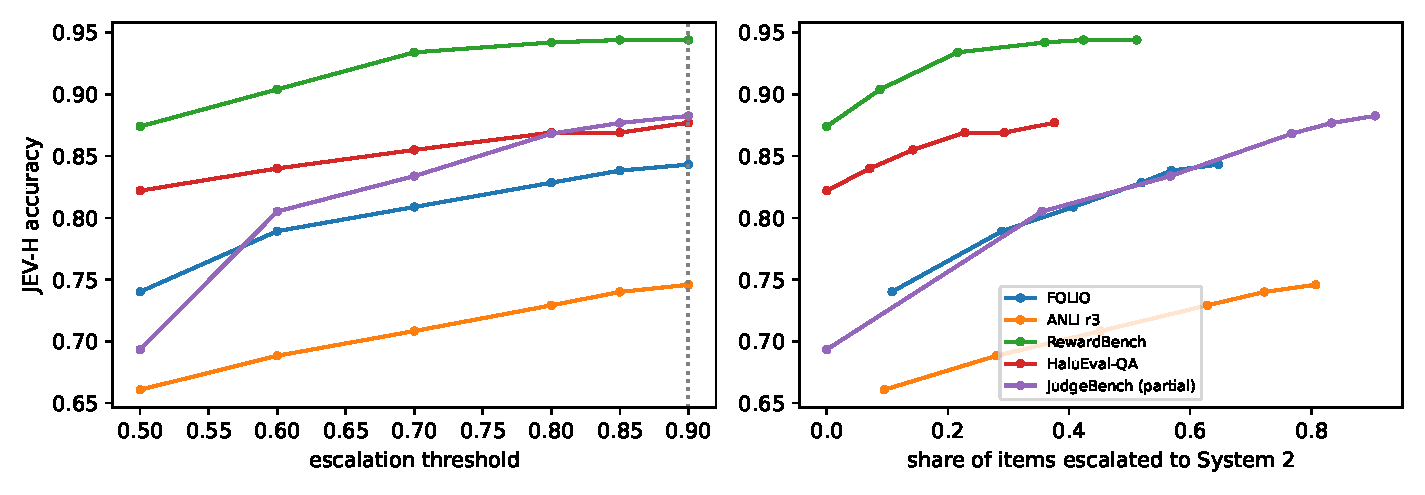
\includegraphics[width=\linewidth]{figures/threshold.pdf}
\caption{JEV-H as the escalation threshold varies (exploratory; the preregistered threshold is 0.90, dotted). Left: accuracy against threshold. Right: accuracy against the share of items escalated to System~2.}
\label{fig:threshold}
\end{figure}
The preregistered threshold of 0.90 was fixed a priori; Figure~\ref{fig:threshold} shows what lower thresholds would have bought, using the System~2 answers already collected.
Most of the gain arrives early: on RewardBench a threshold of 0.70 reaches 93.4\% while escalating 22\% of items (0.90: 94.4\% at 51\%), and on JudgeBench 0.60 already lifts accuracy from 69.3\% to 80.5\% at 36\% escalation.
On FOLIO and ANLI the curve keeps rising to 0.90, because the one-pass model is unsure on most items.
A deployment should choose its threshold from this curve on its own labelled data; \texttt{jevstudy judge} reports it.

\subsection{Robustness}
\label{sec:robust}
\begin{table}[t]
\centering\small
\caption{Option-order reversal (all systems see the reversed list). Flip rate: share of items whose answer, mapped back to the original order, differs from the original answer (\%).}
\label{tab:reversal}
\begin{tabular}{@{}llrrrr@{}}
\toprule
Panel & System & $n$ & Acc.\ orig. & Acc.\ rev. & Flip rate \\
\midrule
FOLIO & JEV-9B S1 & 204 & 69.6 & 68.1 & 5.9 \\
\addlinespace
Controlled base & JEV-9B S1 & 288 & 55.9 & 55.6 & 3.5 \\
\bottomrule
\end{tabular}
\end{table}

Reversing the option list changes System~1's answer on \FlipFolioSone\% of FOLIO items and \FlipCtlSone\% of controlled items (Table~\ref{tab:reversal}), well below the 11.5\% the model card reports for sixteen-option lists; on these three-option tasks position bias is not the main error source.
The frontier arms of this ablation and the max-effort ablation were dropped to limit spending (A5).

\subsection{Can pre-call features say when JEV-9B is enough?}
\label{sec:routing-results}
\begin{table*}[t]
\centering\small
\caption{Selection rules (H3). Leave-one-family-out over five families: mean held-out accuracy (\%), number of folds within 2 points of always-frontier, share of items sent to JEV-9B (\%), and total cost relative to always-frontier. Unseen template: rules fit on everything except controlled template T2, evaluated on T2 items.}
\label{tab:routing}
\begin{tabular}{@{}llrrrrrr@{}}
\toprule
& & \multicolumn{4}{c}{Leave one family out} & \multicolumn{2}{c}{Unseen template T2} \\
Frontier & Policy & Acc. & Within 2 pt & To JEV & Cost ratio & Acc. & To JEV \\
\midrule
Astra & Always JEV-9B & 71.5 & 0/6 & 100 & 0.01 & 49.3 & 100 \\
 & Always frontier & 90.1 & 6/6 & 0 & 1.00 & 100.0 & 0 \\
 & Length only & 90.1 & 6/6 & 1 & 1.00 & 100.0 & 0 \\
 & Family lookup & 90.1 & 6/6 & 0 & 1.00 & 100.0 & 0 \\
 & JEV-9B confidence gate & 87.6 & 4/6 & 45 & 0.67 & 95.1 & 26 \\
 & Feature rule & 87.7 & 4/6 & 19 & 0.84 & 100.0 & 0 \\
 & Feature rule + conf. & 89.3 & 4/6 & 17 & 0.88 & 100.0 & 0 \\
 & Oracle (unattainable) & 93.4 & 6/6 & 78 & 0.25 & 100.0 & 49 \\
\midrule
Fable & Always JEV-9B & 71.5 & 1/6 & 100 & 0.01 & 49.3 & 100 \\
 & Always frontier & 90.9 & 6/6 & 0 & 1.00 & 100.0 & 0 \\
 & Length only & 90.9 & 6/6 & 0 & 1.00 & 100.0 & 0 \\
 & Family lookup & 90.9 & 6/6 & 0 & 1.00 & 100.0 & 0 \\
 & JEV-9B confidence gate & 88.5 & 1/6 & 45 & 0.66 & 95.1 & 26 \\
 & Feature rule & 87.0 & 4/6 & 23 & 0.74 & 100.0 & 0 \\
 & Feature rule + conf. & 88.6 & 4/6 & 21 & 0.78 & 100.0 & 0 \\
 & Oracle (unattainable) & 94.3 & 6/6 & 77 & 0.27 & 100.0 & 49 \\
\bottomrule
\end{tabular}
\end{table*}

Under leave-one-family-out evaluation (Table~\ref{tab:routing}), no rule reaches the always-frontier accuracy band on every held-out family.
Against Astra, the JEV-9B confidence gate keeps \RouteAstraGateAcc\% mean held-out accuracy (always-Astra: \RouteAstraAfrAcc\%) at \RouteAstraGateCost{} of the cost, and is within two points of always-Astra on \RouteAstraGateWithin{} folds; the feature rule plus confidence reaches \RouteAstraRuleconfAcc\% at \RouteAstraRuleconfCost{} of the cost (\RouteAstraRuleconfWithin{} folds).
Length-only and family-lookup rules degenerate to always-frontier on held-out families.
H3 is therefore only partly supported: features add a little to the confidence gate, neither reliably preserves frontier accuracy on a family it was not fit on, and the oracle (\RouteAstraOracleAcc\% at \RouteAstraOracleCost{} of the cost) shows how much routing headroom remains.

\subsection{Bridge to official Jev}
\label{sec:bridge}
\begin{table}[t]
\centering\small
\caption{ProofWriter bridge (A2, exploratory). JEV-9B~S1 accuracy (\%) on 900 open-world items (50 per depth $\times$ label) with Hard-Decisions' task wording, beside official Jev, Kev-9B and GPT-6 Luna (reasoning off) as published by Hard-Decisions on a different sample of the same strata. JEV-9B by label: true 54.2, false 57.3, unknown 71.1.}
\label{tab:bridge}
\begin{tabular}{@{}rrrcrrr@{}}
\toprule
Depth & $n$ & JEV-9B S1 & 95\% CI & Official Jev & Kev-9B & Luna (off) \\
\midrule
0 & 150 & 94.0 & [89.0, 96.8] & 97.7 & 89.3 & 93.3 \\
1 & 150 & 72.7 & [65.0, 79.2] & 87.7 & 73.8 & 77.8 \\
2 & 150 & 57.3 & [49.3, 65.0] & 84.8 & 58.4 & 60.4 \\
3 & 148 & 56.8 & [48.7, 64.5] & 79.9 & 49.5 & 61.7 \\
4 & 149 & 42.3 & [34.6, 50.3] & 71.9 & 38.6 & 44.6 \\
5 & 143 & 40.6 & [32.9, 48.8] & 81.0 & 41.2 & 46.0 \\
\bottomrule
\end{tabular}
\end{table}

\begin{figure}[t]
\centering
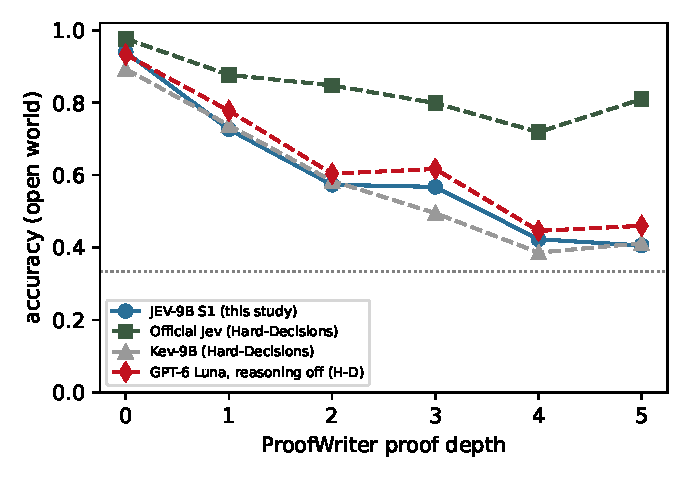
\includegraphics[width=0.62\linewidth]{figures/bridge.pdf}
\caption{ProofWriter open-world accuracy by proof depth: JEV-9B~S1 (this study, 900 items) against official Jev, Kev-9B and GPT-6 Luna without reasoning as published by Hard-Decisions on a different sample of the same strata.}
\label{fig:bridge}
\end{figure}
On ProofWriter (A2, exploratory), JEV-9B falls from \BridgeDZero\% at depth~0 to \BridgeDFive\% at depth~5 (Table~\ref{tab:bridge}, Figure~\ref{fig:bridge}).
Official Jev, on a different sample of the same strata, falls only to 81.0\%.
At depth~0 the student is within four points of its teacher; from depth~2 on it tracks Kev-9B, a different 9B decision model, and not Jev.
\textbf{This is the most important qualification of everything above}: the student's reasoning-depth behaviour is not the teacher's, so our negative results about JEV-9B on reasoning panels should not be read as results about official Jev.
